\chapter[Dashboard]{Dashboard}
O objetivo deste capítulo é descrever a solução, a qual tem como objetivo atender às necessidades colocadas no primeiro capítulo, referente à problemática deste trabalho. A apresentação da solução está concentrada em três partes. A primeira parte está relacionada à coleta das métricas utilizando a ferramenta SonarQube, e a segunda parte está relacionada à criação do \textit{dashboard} e à visualização das informações. A terceira e última parte da solução, consiste na análise dos resultados obtidos através de uma avaliação qualitativa com possíveis usuários.

\section{Ambiente Simulado}
Para se simular um ambiente de produção, foi utilizado como modelo de referência o ambiente apresentado por Luiza e Yago \cite{luiza_yago}. No trabalho descrito, os autores caracterizam o Órgão pertencente à APF como Órgão X. Uma das características referentes ao Órgão X que podem ser citadas diz respeito a sua área de jurisdição que abrange serviços de radiodifusão, postais e de telecomunicações. O Órgão X atualmente implanta o GeDDAS (Gestão de Demandas de Desenvolvimento Ágil de Software) proposto por Souza \cite{souza_sobrinho_uso_2014}. A Figura \ref{img:proc_des} apresenta o processo de desenvolvimento adotado pelo Órgão X. Uma vez definido como seria o ambiente simulado, comecou-se a elaborar o conceito do \textit{dashboard}.

\graphicspath{{figuras/}}
\begin{figure}[h!]
\centering
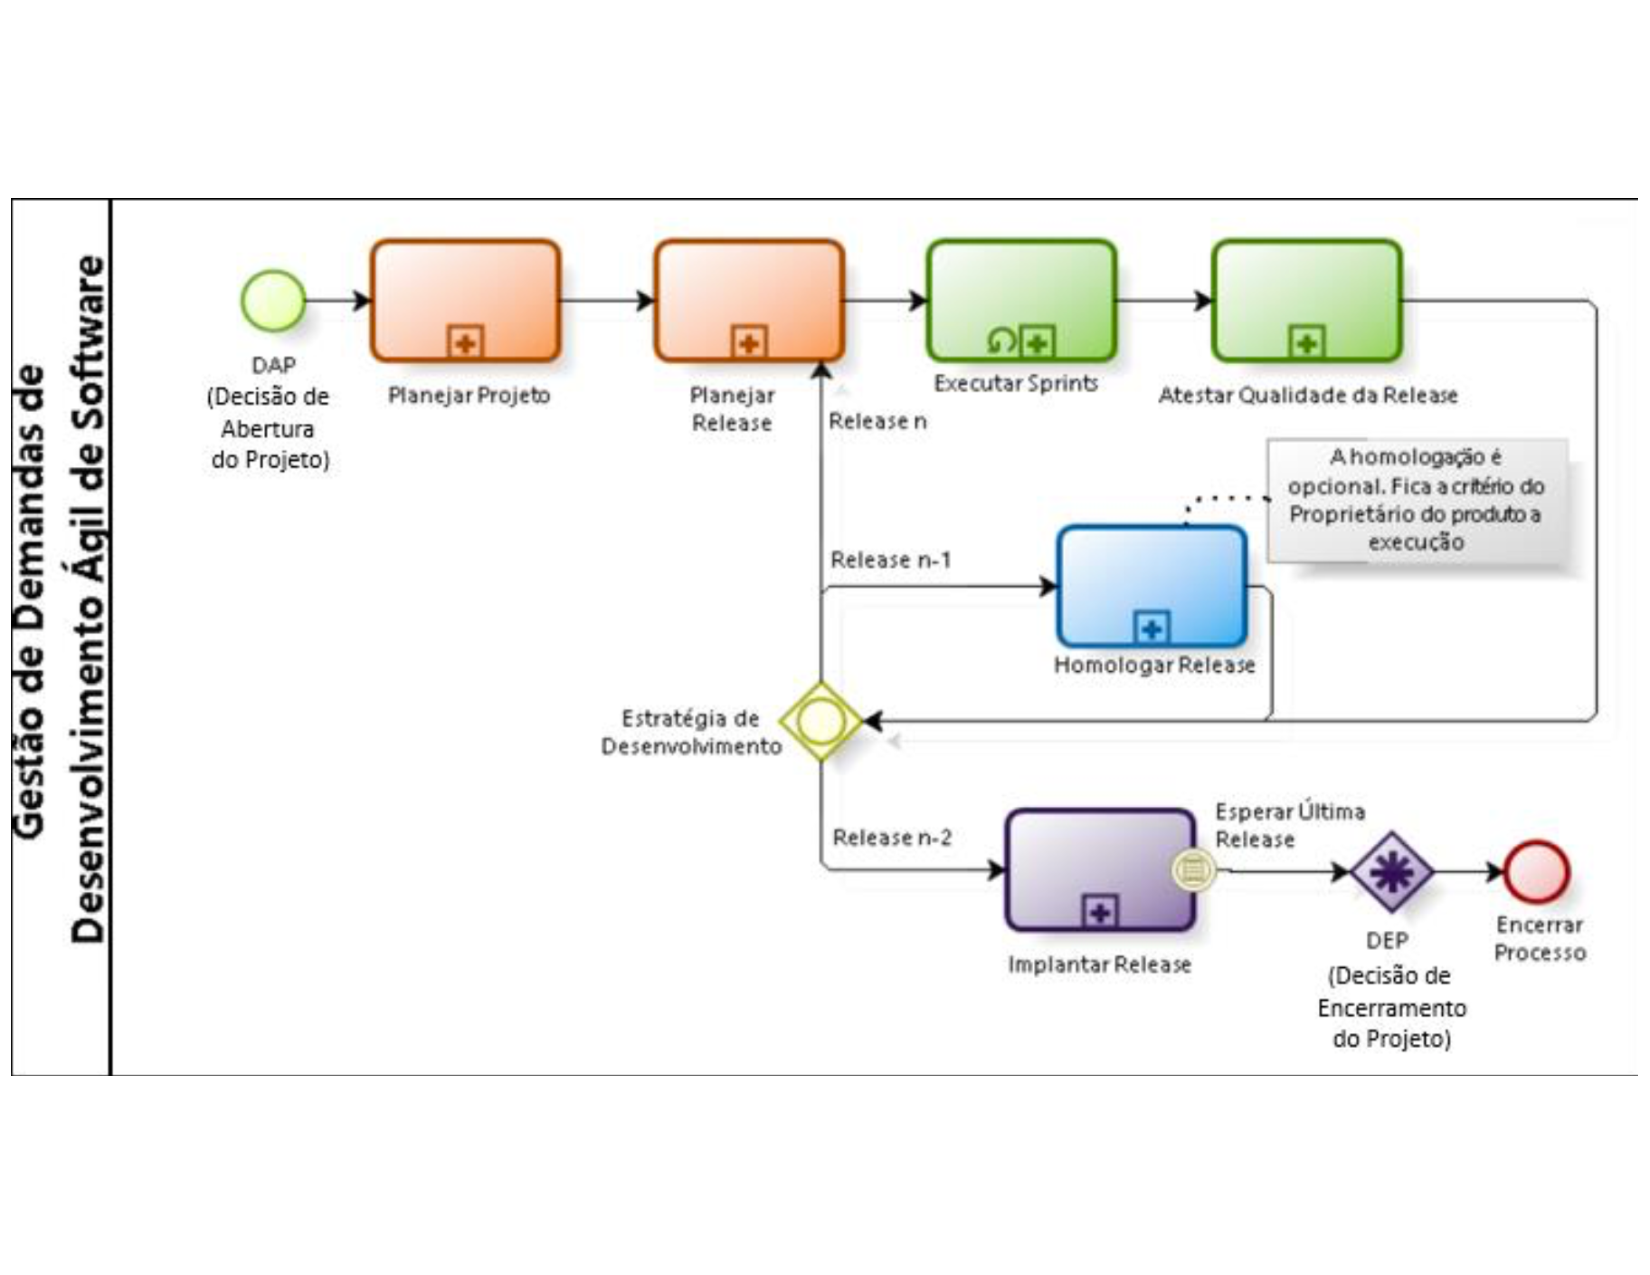
\includegraphics[scale=0.60]{Proc_des.pdf}
\caption{Processo de Desenvolvimento Adotado Pelo Órgão X. Fonte: \cite{luiza_yago}}
\label{img:proc_des}
\end{figure}

A solução tem o objetivo de atuar tanto do lado do Órgão Público, onde o Gestor acompanha o desenvolvimento do projeto, quanto da empresa contratada em que a ferramenta é integrada ao processo de desenvolvimento do software. A Figura \ref{img:ciclo_ver} apresenta um diagrama que demonstra o ciclo de verificação juntamente com a solução apresentada. Na Figura é possível observar que o time de desenvolvimento, da empresa contratada, desenvolve o código que é submetido para uma análise, onde é feita a verificação das métricas que foram estipuladas. Após essa análise o resultado é submetido para o \textit{dashboard},  dessa forma, tanto o Gestor de TI quanto a equipe de qualidade do Órgão, podem acompanhar o projeto. 

\graphicspath{{figuras/}}
\begin{figure}[!]
\centering
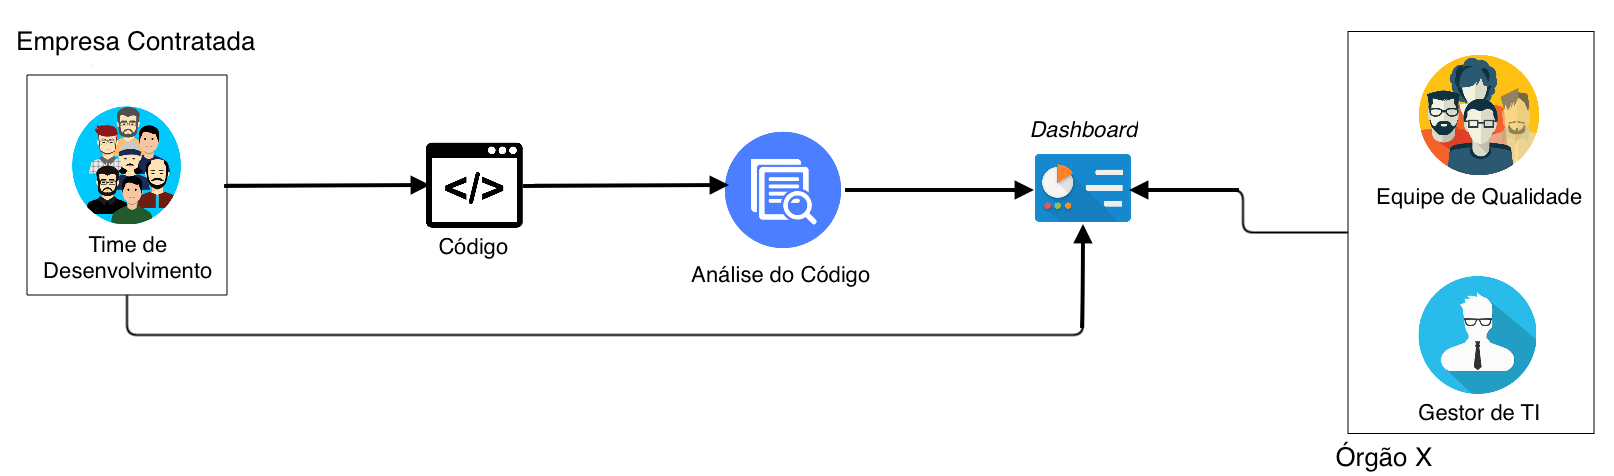
\includegraphics[scale=0.30]{proc_ver.png}
\caption{Ciclo de Verificação Utilizando a Solução Compartilhada Entre Órgão Contratante e Empresa Contratada}
\label{img:ciclo_ver}
\end{figure}


\section{Criação do \textit{Dashboard}}

Antes da criação do \textit{dashboard} era necessário entende quais seriam os seus requisitos. Para coletar os requisitos funcionais foram elaborados um conjunto de histórias de usuário, está técnica é proposta pelo Scrum para auxiliar no entendimento dos requisitos. Foram definidas cinco histórias que contemplam o funcionamento de todo o sistema. As histórias estão presentes na tabela \ref{tabela_historia} juntamente com os seus critérios de aceitação. Com as histórias definidas, foram feitas algumas telas para auxiliar tanto no entendimento das funcionalidades quanto na escrita das histórias. 

\begin{table}[]
\centering
\caption{Histórias de Usuários Que Foram Definidas}
\label{tabela_historia}
\begin{tabular}{|l|l|l|}
\hline
\rowcolor[HTML]{C0C0C0} 
\textbf{\#} & \textbf{História de Usuário}                                                                                                                                                                                       & \textbf{Critério de Aceitação}                                                                                                                                                                                                                                                          \\ \hline
1           & \begin{tabular}[c]{@{}l@{}}Eu como gestor quero\\ realizar o login na apli-\\ cação, para poder cadas-\\ trar projetos\end{tabular}                                                                                & \begin{tabular}[c]{@{}l@{}}1. Tela de login com campo \\ “Usuário”e “Senha”.\\ 2. O campo “Usuário” deve \\ ser único e conter o email \\ do gestor.\\ \\ \\ 3. O campo “Senha” deve ser \\ formado com no mínimo oito \\ caracteres sendo pelo menos \\ um em Caixa Alta.\end{tabular} \\ \hline
2           & \begin{tabular}[c]{@{}l@{}}Eu como gestor desejo \\ gerenciar projetos para\\ que possa acompanha-\\ los de maneira mais or-\\ ganizada\end{tabular}                                                               & \begin{tabular}[c]{@{}l@{}}1. É necessário ter as funcio-\\ nalidades de: cadastrar, alterar\\  e excluir projeto.\end{tabular}                                                                                                                                                         \\ \hline
3           & \begin{tabular}[c]{@{}l@{}}Eu como gestor desejo \\ visualizar em forma de\\ widgets um resumo de\\ cada projeto na tela \\ inicial do software para \\ simplificar o acompanha\\ mento dos projetos.\end{tabular} & \begin{tabular}[c]{@{}l@{}}1. Na tela principal deve existir\\ widgets relacionados que tragam\\  um breve resumo dos projetos re-\\ ferentes àquele gestor.\end{tabular}                                                                                                               \\ \hline
4           & \begin{tabular}[c]{@{}l@{}}Eu como gestor gostaria \\ de sugestões de métricas \\ para os meus projetos.\end{tabular}                                                                                              & \begin{tabular}[c]{@{}l@{}}1. O sistema deve sugerir mé-\\ tricas para o gestor.\\ 2. Essas métricas devem ter \\ relação ou com o perfil do \\ gestor ou com o projeto em \\ desenvolvimento.\end{tabular}                                                                             \\ \hline
5           & \begin{tabular}[c]{@{}l@{}}Eu como gestor desejo \\ utilizar mais de uma \\ aplicação de análise \\ estática para caso haja \\ uma eventual migração \\ de ferramenta.\end{tabular}                                & \begin{tabular}[c]{@{}l@{}}1. Deve ser possível cadastrar \\ novas ferramentas de análise \\ estática, contanto que elas sigam\\  os padrões esperados.\\ 2. Deve haver uma tela para \\ cadastro de novas ferramentas.\end{tabular}                                                    \\ \hline
\end{tabular}
\end{table}

A Figura \ref{img:telaLogin} apresenta a tela inicial da solução, por onde o Gestor fará o acesso colocando seu \textit{usuário} e sua \textit{senha}. Ainda nesta tela, existe um \textit{link} para caso o Gestor não se lembre da sua \textit{senha}, neste caso o sistema enviará uma mensagem para o \textit{email} cadastrado pelo gestor, solicitando a alteração.

\graphicspath{{figuras/}}
\begin{figure}
\centering
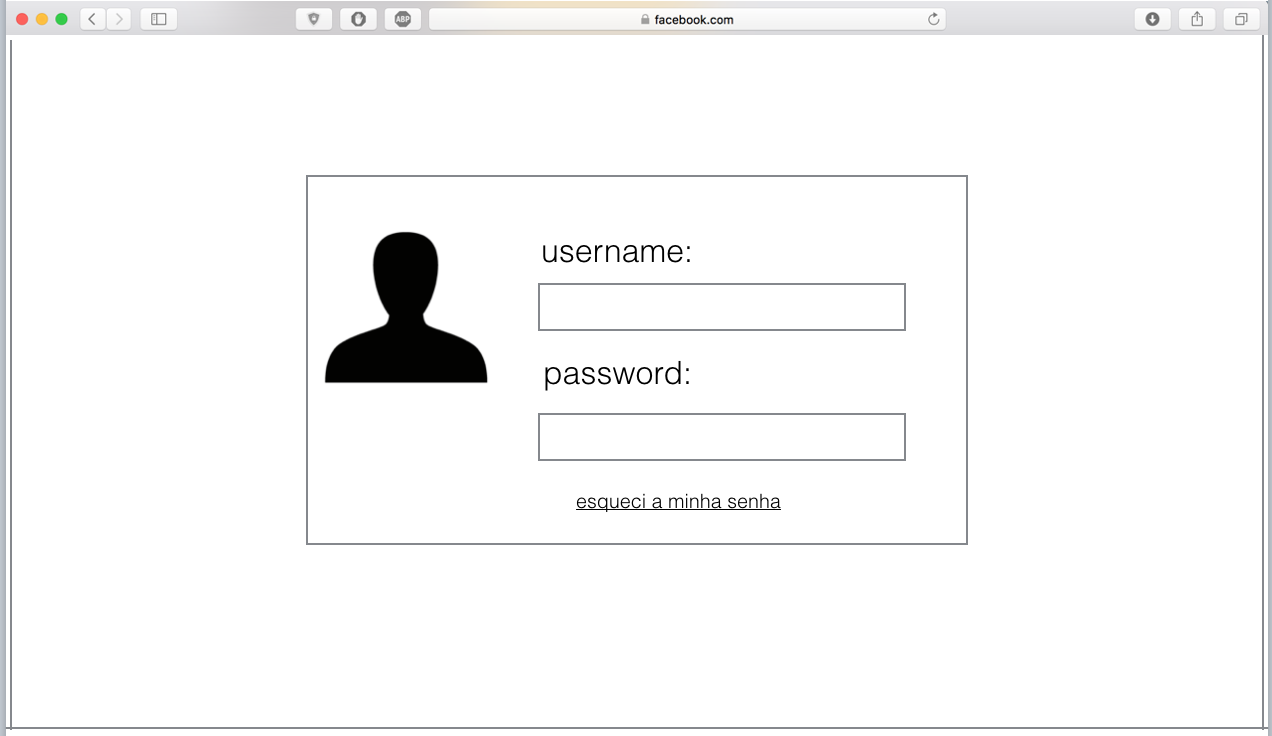
\includegraphics[scale=0.60]{telaLogin.png}
\caption{Tela Login}
\label{img:telaLogin}
\end{figure}

A página inicial da solução é apresentada na Figura \ref{img:telaHome}. Nesta página, o Gestor tem uma visão de todos os projetos, que ele cadastrou para serem acompanhados. Cada projeto é representado por um retângulo de uma cor , e neste retângulo estão algumas informações referentes ao projeto, que podem ser visualizadas, sem a necessidade de se abrir o projeto. Tanto as cores dos retângulos, como as informações dos projetos podem ser alteradas de acordo com o Gestor. Nesta página, ainda existe um botão que direciona o usuário para a tela de "adicionar projetos". Esta tela é somente para o gestor.
 
\graphicspath{{figuras/}}
\begin{figure}
\centering
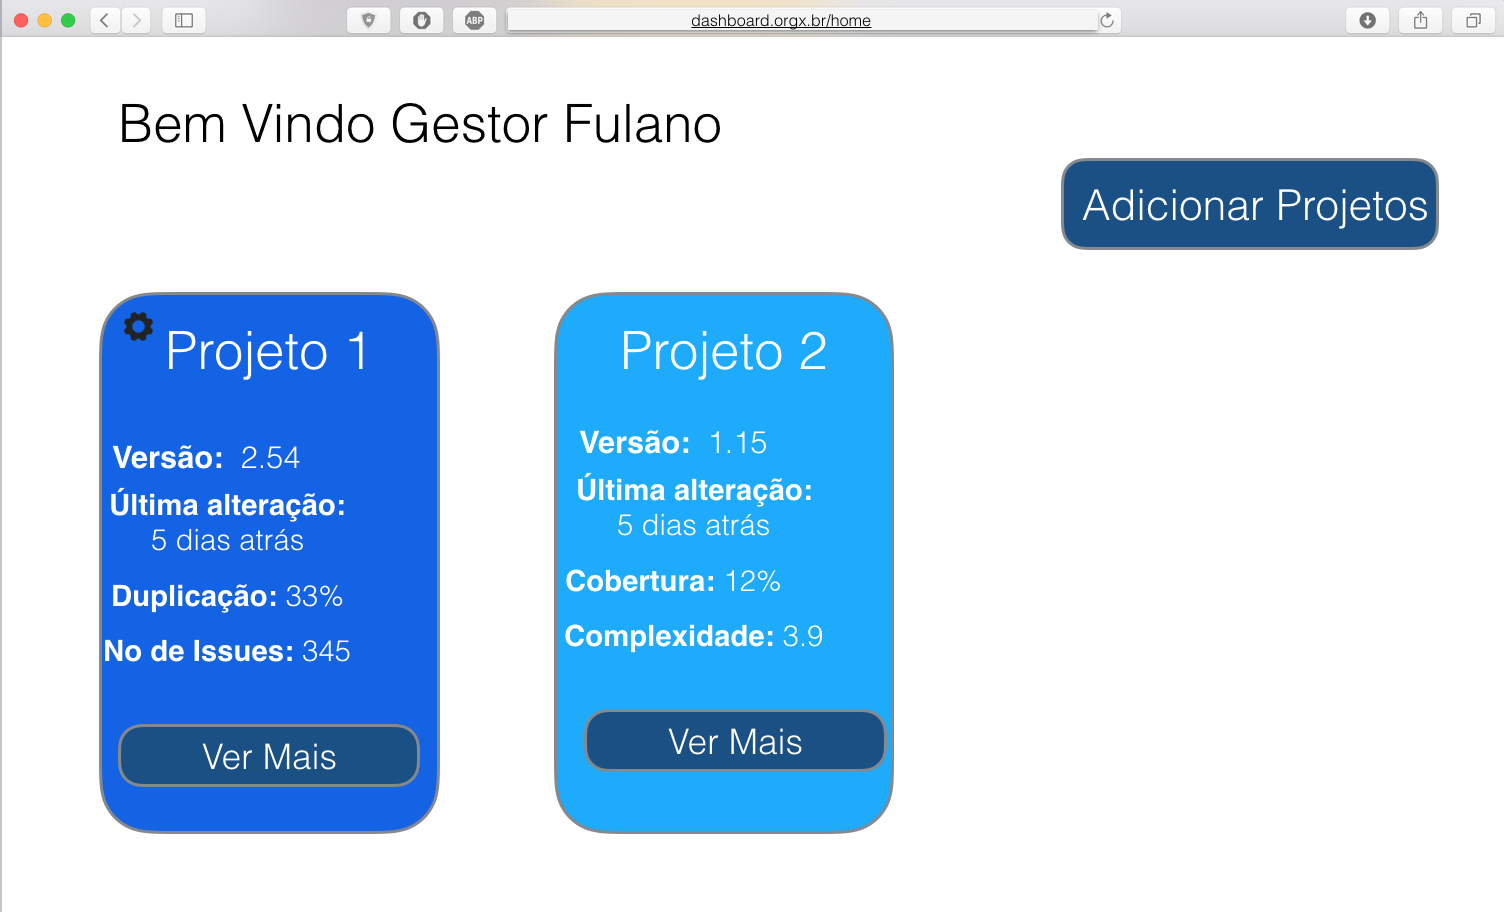
\includegraphics[scale=0.60]{telaHome2.png}
\caption{Tela Home}
\label{img:telaHome}
\end{figure} 

A Figura \ref{img:telaDashboard} apresenta um protótipo do \textit{dashboard} que será implementado. Nesta página encontram-se as informações referentes ao projeto selecionado. Está página apresenta em forma de gráficos, as métricas que foram selecionadas pelo Gestor para aquele projeto. Esta é a única página que pode ser acessada pela empresa terceirizada. Em cada métrica é possível passar colocar a seta do \textit{mouse} por cima do ícone "?" para que se tenha uma breve explicação da métrica 

\graphicspath{{figuras/}}
\begin{figure}
\centering
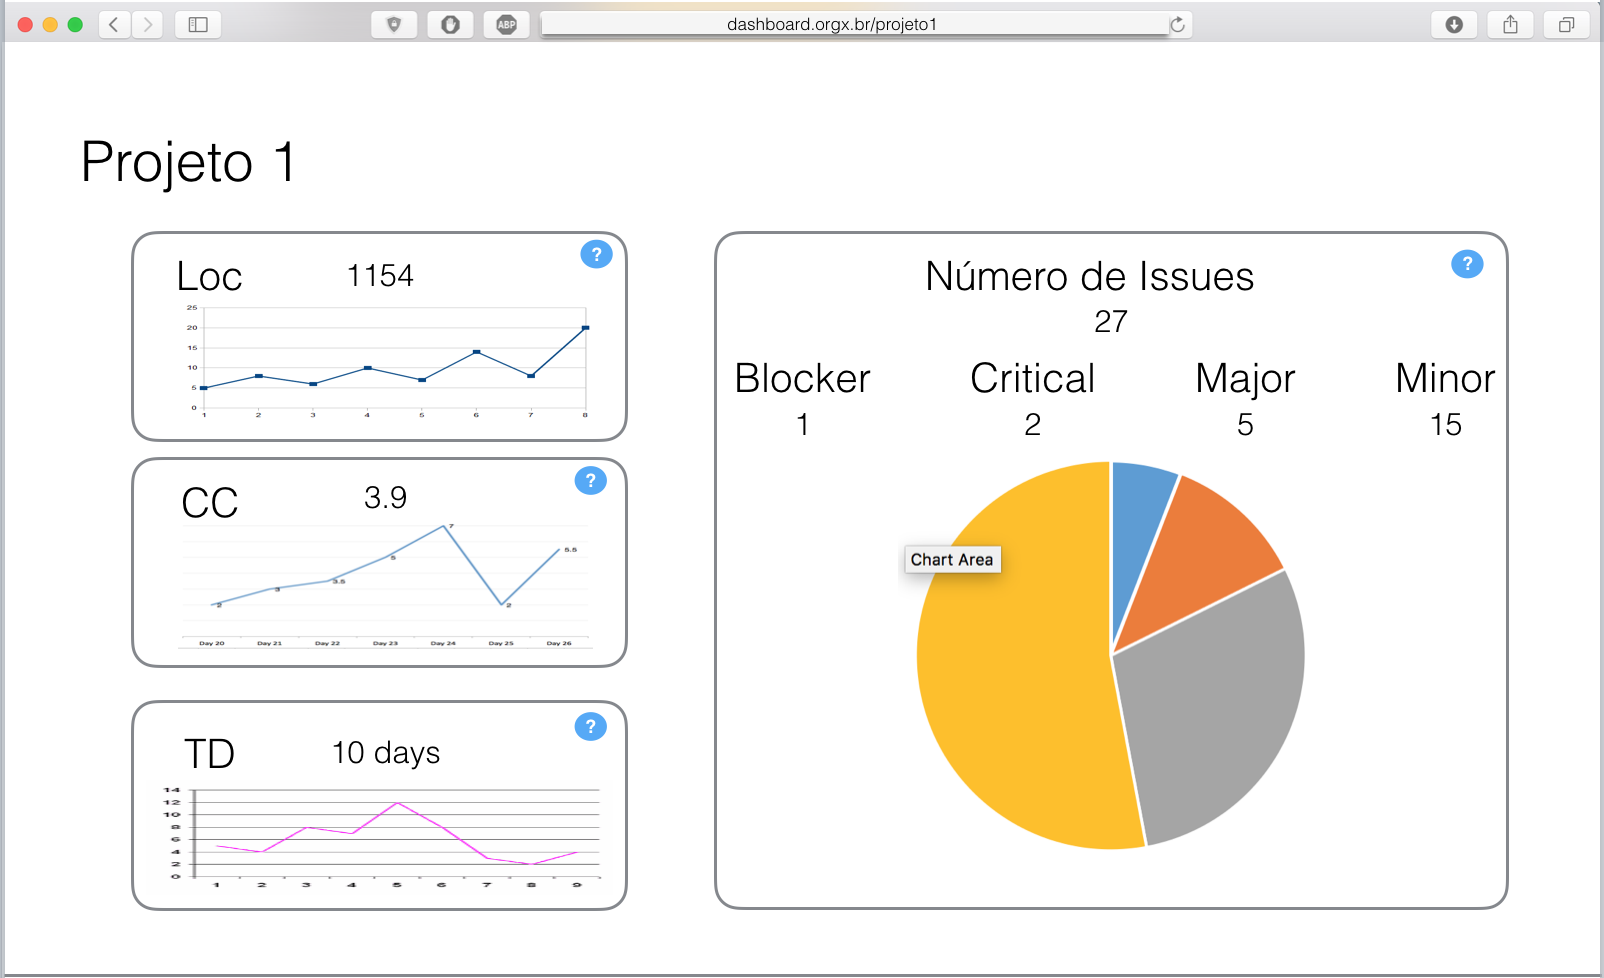
\includegraphics[scale=0.60]{telaDashboard.png}
\caption{Tela \textit{Dashboard}}
\label{img:telaDashboard}
\end{figure} 

Para se fazer a adição de um novo projeto, é necessário que o projeto a ser adicionado, esteja armazenado em um repositório que o Gestor tenha acesso de leitura. A Figura \ref{img:telaAdicionar} representa um protótipo da página de adição de projetos. Nesta página são adicionados, o nome do projeto, uma descrição, a url do repositório em que se encontra o projeto e por último, as métricas que serão analisadas. Assim como na página do \textit{dashboard}, cada métrica apresenta um ícone "?" que apresenta uma breve explicação de cada métrica.

\graphicspath{{figuras/}}
\begin{figure}
\centering
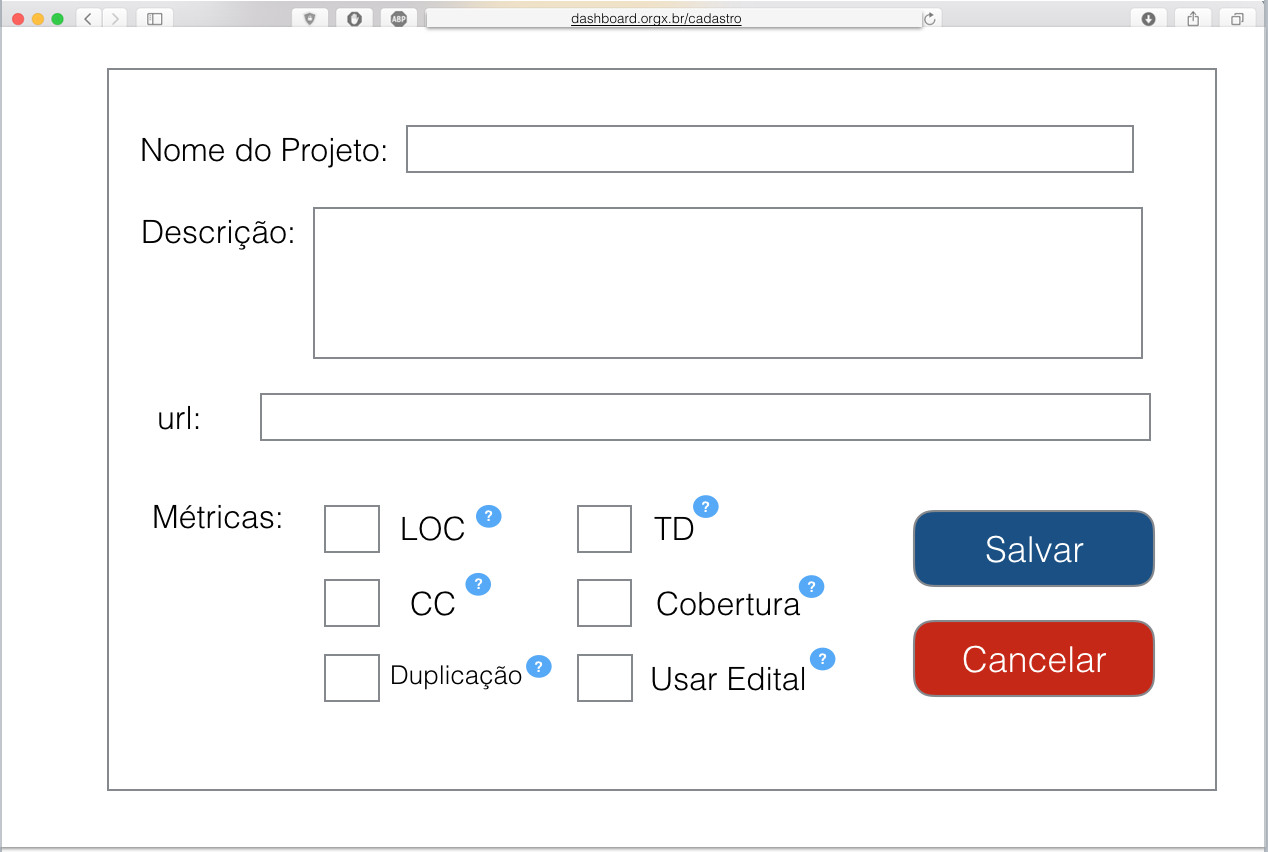
\includegraphics[scale=0.60]{telaAdicionar.png}
\caption{Tela Adicionar}
\label{img:telaAdicionar}
\end{figure} 

Com as histórias definidas e um protótipo de como deveria funcionar o sistema começou-se a planejar as \textit{sprints} de acordo com o nível de importância da funcionalidade para a aplicação como um todo. Dividiu-se da seguinte forma:

\begin{itemize}
\item\textit{Sprint 1}: História  de Usuário 1
\item\textit{Sprint 2}: Histórias  de Usuário 2 e 3
\item\textit{Sprint 3}: História  de Usuário 5
\item\textit{Sprint 4}: História  de Usuário 4
\end{itemize}

Uma das principais funcionalidades do \textit{dashboard} é a coleta das métricas e a sugestão dessas métricas. Por esse motivo foi dedicado um tempo maior nas \textit{sprints} para implementação dessas funcionalidades.   

\section{Coleta e Sugestão das Métricas}

Para fazer a coleta das métricas, foi utilizado a ferramenta SonarQube juntamente com a ferramenta Codacy como forma de elucidação de uma possível expansão que pode ser feita no software. A sugestão das métricas utiliza o conceito do algoritmo de aprendizado de maquina, que sugere que o gestor avalie de 0 a 100, três métricas distintas de acordo com o quão necessário ele acredita ser aquela métrica para aquele projeto. Baseado nessa sugestão o algoritmo interpola os dados inseridos pelo usuário, juntamente com um conjunto de quatro \textit{Personas} com características específicas. Através do cruzamento dos perfis, o algoritmo sugere um conjunto de métricas baseado no perfil mais semelhante ao do usuário. A Figura \ref{img:perfis} apresenta de maneira simplificada como será o cruzamento dos dados entre as \textit{Personas} e o Usuário.

\graphicspath{{figuras/}}
\begin{figure}[h!]
\centering
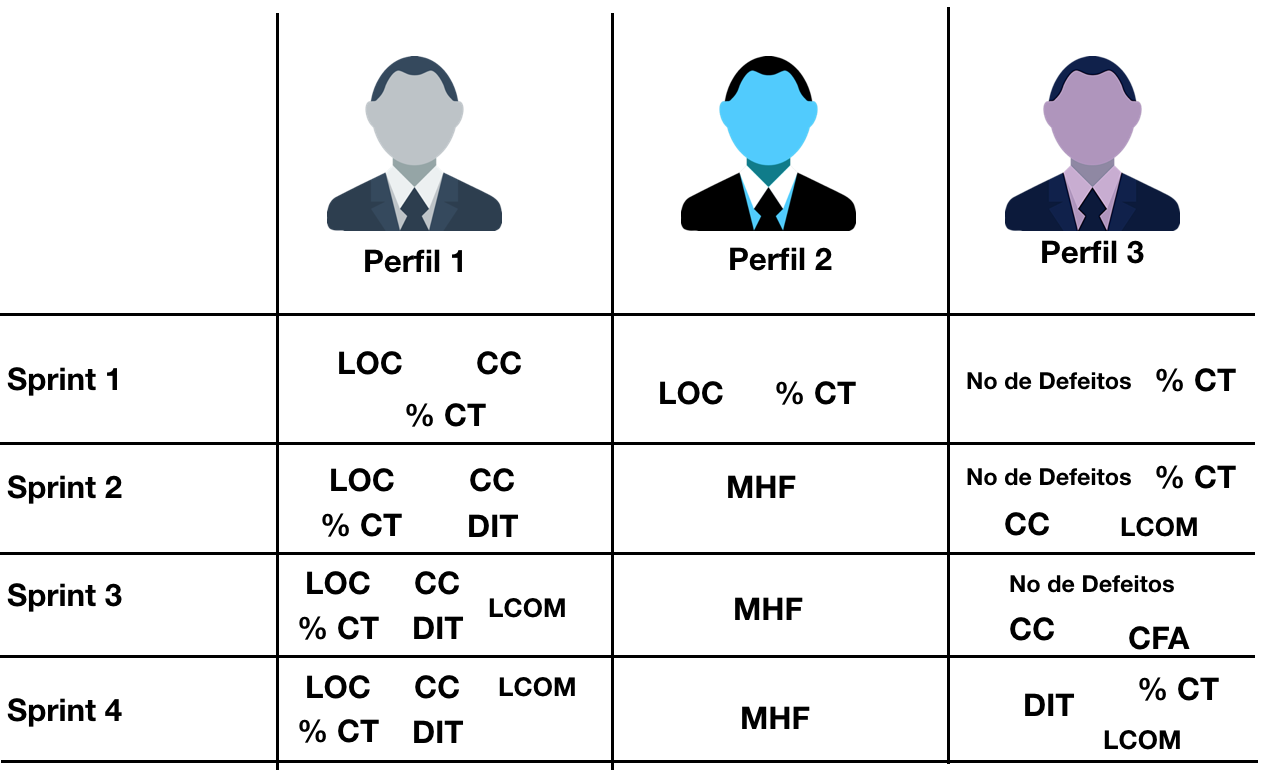
\includegraphics[scale=0.50]{perfis_exemplo.png}
\caption{Exemplo de Perfis Coletados Após Questionário}
\label{img:perfis}
\end{figure}

O objetivo deste trabalho é criar uma ferramenta que auxilie na auditoria de produtos de software entregues por empresas terceirizadas. Entretanto dificilmente o mesmo irá substituir o fator humano da auditoria. Portanto, o software compreende apenas um suporte, que visa facilitar a avaliação geral do software entregue sob o ponto de vista da qualidade de código. Recomenda-se que o software seja submetido à ferramenta e seja aceito, a realização de uma auditoria em cima de uma amostragem do software entregue, sob o olhar de um analista especializado para tal atividade.

Foi elaborado uma prova de conceito, para que se pudesse testar a funcionalidade relacionada à coleta de métricas. Está prova, consiste em, elaborar um software que fosse capaz de extrair métricas do relatório do SonarQube. Inicialmente foi necessário criar uma instância do SonarQube e fazer a análise de um projeto. O projeto escolhido foi um projeto em Java, que o próprio SonarQube disponibiliza para download, com o intuito de ser utilizado como exemplo. Com o ambiente configurado, implementou-se uma solução em Python que atendesse aos requisitos estabelecidos para a prova de conceito. A Figura \ref{img:terminal} apresenta a saída do console, ao se rodar a solução.


\graphicspath{{figuras/}}
\begin{figure}[H]
\centering
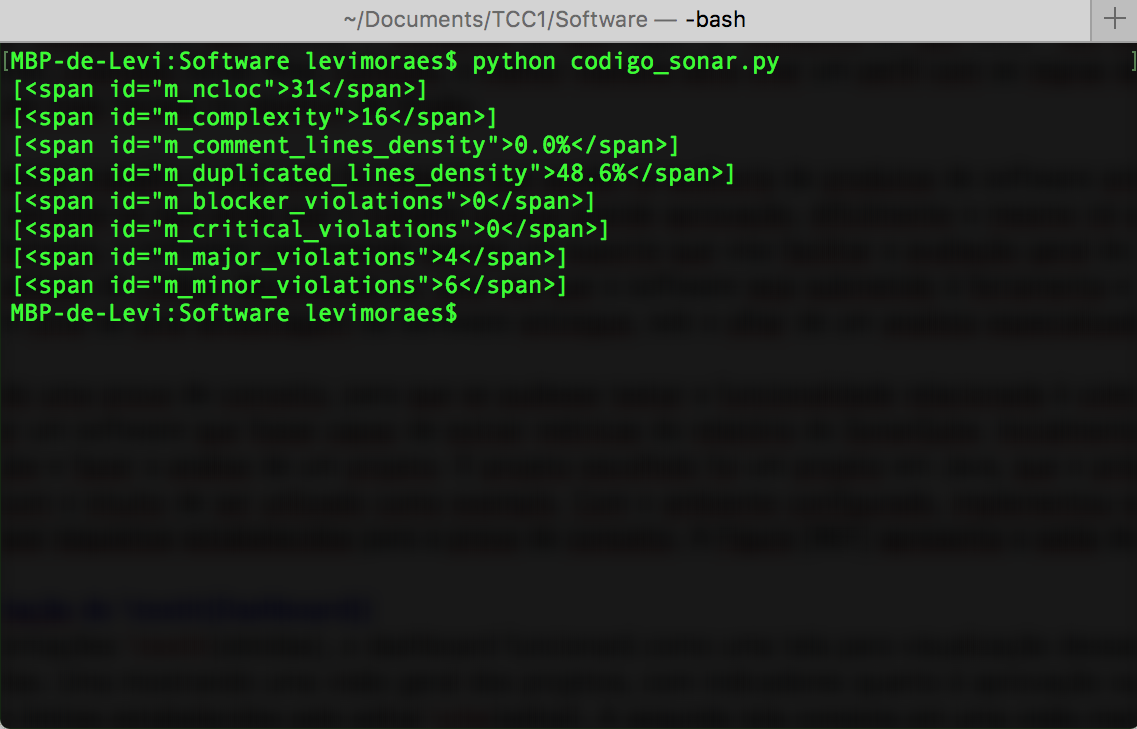
\includegraphics[scale=0.60]{terminal.png}
\caption{Métricas Extraídas do SonarQube}
\label{img:terminal}
\end{figure}


A ultima parte do \textit{dashboard} consiste na avaliação que foi feita ao fim de cada etapa do desenvolvimento. Essa avaliação tem por objetivo garantir que o software que estava sendo entregue atendia aos requisitos propostos inicialmente. 


\section{Avaliação}

A avaliação do \textit{dashboard} foi feita por um grupo de usuários que não trabalham no Órgão X. Essa avaliação foi conduzida em um período de três iterações. Nestas iterações foram avaliados aspectos de usabilidade da ferramenta e se a ferramenta possuía condições mínimas de ser implantada. Na primeira iteraçao foram feitas as seguintes perguntas, sempre anotando o tempo de execução e avaliando a experiência do usuário
\begin{enumerate}
\item Você consegue realizar um cadastro ?
\item Você consegue realizar um \textit{login}, utilizando o usuário que você criou ?
\item Você consegue criar um projeto com as seguintes características ?1:30

Nome do Projeto: Arma-X
Descrição do Projeto: Projeto para exterminação da raça humana
Data de Início: 25/01/2017
Data de Término: 25/12/2017
Linguagem: PHP
Métricas: LOC e IRA
\textit{Widget} do tipo 2

\item Você consegue listar todos os seus projetos em uma única tela ?
\item Você consegue exibir informações do seu projeto ?
\item Algum dos gráficos exibidos lhe parece não-familiar, ou causa estranheza ?
\item Se você tivesse que escolher um dos gráficos para determinar uma nota geral para o projeto, você escolheria algum desses ?
\end{enumerate}

Coletados os resultados e após a implementação de novas funcionalidades, foram feitas novas avaliações. Para a segunda iteração foram feitas as seguintes perguntas: 

\begin{enumerate}
\item Você consegue acessar o calendário ?
\item Você consegue criar um evento para o dia 01/11 ?
\item Você consegue voltar para o menu ?
\item Você sabe dizer em que linguagem foi escrito o projeto Arma-X ?
\item Você consegue me dizer a porcentagem de duplicação na versão 1.3 ? 
\item Você consegue me explicar o que são \textit{issues} ?
\item  Você consegue me dizer o repositório Github do projeto ?
\end{enumerate}

Na última iteração foi pedido aos entrevistados que respondessem a um questionário elaborado segundo o modelo do SUS, relatando a experiência deles com o software. O objetivo dessa avaliação é para que se tenha quantificado o nível de usabilidade do software entregue. A coleta do questionário foi feita utilizando o Google Forms, onde o questionário era enviado por \textit{email} para os usuários e ao responder a ferramenta armazenava a resposta. Seguindo o modelo do questionário SUS, foram feitas as seguintes perguntas:

\begin{enumerate}
\item Eu acho que gostaria de usar esse sistema com frequência.
\item Eu acho o sistema desnecessariamente complexo.
\item Eu achei o sistema fácil de usar.
\item Eu acho que precisaria de ajuda de uma pessoa com conhecimentos técnicos para usar o sistema.
\item Eu acho que as várias funções do sistema estão muito bem integradas.
\item Eu acho que o sistema apresenta muita inconsistência.
\item Eu imagino que as pessoas aprenderão como usar esse sistema rapidamente.
\item Eu achei o sistema atrapalhado de usar.
\item Eu me senti confiante ao usar o sistema.
\item Eu precisei aprender várias coisas novas antes de conseguir usar o sistema.
\end{enumerate}

\section{Resumo do Capítulo}

A proposta deste trabalho é criar uma maneira facilitada de acompanhar a qualidade de código estático dos produtos de software entregues pelas terceirizadas. Para fazer esta análise, a solução orienta-se por uma ferramenta de análise estática SonarQube, e por um conjunto de métricas relacionadas às boas práticas de programação encontradas na ferramenta Codacy. A solução encontrada foi a utilização de um \textit{dashboard} que através de um algoritmo de sugestão, auxilie o gestor no acompanhamento de um projeto, e que através dessas métricas, fosse possível aferir a qualidade do código para aquele projeto. A última etapa deste \textit{dashboard}, consiste em um conjunto de testes de usabilidade. Durante três iterações foram avaliados aspectos de usabilidade e aplicabilidade da solução proposta em um ambiente real.